\chapter{Application to railway conflict management}

As the last point in the thesis, in this chapter we describe how the results presented so far can be
applied in the field of operational research. Namely, we propose an approach to solving the railway
dispatching problem using quantum annealing. We benchmark the implementation of our algorithm on the
current generation of D-Wave annealers, using solutions obtained via tensor networks and exhaustive
search as a baseline for comparison.


\section{Overview of the problem}
Before formulating the problem to be solved, let us first introduce the necessary railway--related
terminology. We will consider a part of a railway network, which we will simply refer to as a
\emph{network}. The network is divided into \emph{block sections}. In our work, we focused only on
the single--track railways, which means that the network can only comprise the following types of
sections:
\begin{itemize}
    \item Single tracks, sections that can be occupied by one train at a time.
    \item Sidings, or parallel tracks (occurring e.g. at stations). At the sidings, trains passing in
        the same direction can meet and overtake, and trains passing in the opposite directions can
        meet and pass. Each siding comprises two or more tracks, each of which can also be occupied by
        one train at a time.
\end{itemize}

Fig. \ref{fig:railway-network} shows an example network studied in our work. The trains move through
the network according to a \emph{timetable}. It is assumed that this timetable is conflict-free.
That is, at any time no two trains occupy the same block section, except possibly at sidings (where
the number of trains does not exceed the number of tracks in the siding).

Now, suppose the network is affected by a disturbance, which prevented some trains from running
according to their original timetable. Examples of possible disturbances include (but are not
limited to) a malfunction of one or more trains or a malfunction of railway tracks.
After the disturbance, some trains occupy different parts of the networks than they are supposed to
occupy. Resuming operations according to the original timetable could result in a conflict. Hence,
after the disturbance, a new, conflict--free timetable has to be promptly created. Optimally, this
new timetable should, in some sense, minimize the resulting delays.

Let us observe that even with the best possible algorithm for constructing a new timetable, some
delays after the disturbance might be inevitable, e.g. due to engineering or even physical limits.
For instance, if a train was unable to move for a few hours, it is obvious that it will not reach
its destination on schedule. These unavoidable, or \emph{primary}, delays propagate through the
network and cannot be mitigated. There are also \emph{secondary} delays, i.e. delays that are
introduced in the network because of the restrictions on the new timetable (e.g. necessity of
avoiding conflicts). Differentiating between those two components of delays is crucial because it
allows us to neglect the primary delays and focus only on secondary details when constructing the
objective function.

\section{Railway model and basic notation}
Let us now expand on the informal description from the previous section. We will start by introducing
notation and the definitions necessary to formulate a problem in such a way that it can be run on D-Wave.

Before we can formulate the optimization problem at hand in a way that it can be run on D-Wave, let
us introduce the needed notation. The set of all trains will be denoted by $\JJ$. This set is
naturally partitioned into the set $\JJ_0$ of trains going into one direction and set $\JJ_1$ of
trains going into the opposite direction. This is a proper partition, i.e.
\begin{equation}
	\JJ_0 \cup \JJ_1 = \JJ \quad \JJ_0 \cap \JJ_1 = \emptyset
\end{equation}

For any train, $j \in \JJ$ its route $M_j$ is a sequence of blocks. Our model forbids recirculation,
i.e. each train passes every block in its route exactly once. Furthermore, we assume that each train
starts and ends its route at some station, and its route is uniquely identified by a sequence of
station blocks $\left(s_{j,1}, s_{j, 2}, \ldots, s_{j, \mbox{end}_j}\right)$. In other words, there
are no alternative routes between any two stations. For convenience, we will denote the block
preceding $s_{j,k}$ in a given train's route by $\pi(s_{j,k})$ and the block succeeding it by
$\rho(s_{j,k})$, i.e.
\begin{align}
	\pi(s_{j,k})  & = s_{j,k-1} \quad \mbox{for } 2 \le k \le \mbox{end}_j      \\
	\rho(s_{j,k}) & = s_{j,k+1} \quad \mbox{for } 1 \le k \le \mbox{end}_j - 1.
\end{align}
We will denote the time at which the train $j$ should leave the block $s$ according to the original
timetable by $\ttout(j, s)$. Similarly, the time at which the train $j$ is supposed to leave block $s$
will be denoted by $\ttin(j, s)$. In our model, we assume that the time at which a train leaves one
block is precisely the same as the time it enters the next block, i.e.
\begin{equation}
	\ttout(j, s) = \ttin(j, \rho_j(s))
\end{equation}
It is clear that the original timetable determines how long it takes for a train $j$ to travel
through a given block $s$. We call this time the passage time, denoted by $\pt(j, s)$
\begin{equation}
	\pt(j, s) = \ttout(j, s) - \ttin(j, s)
\end{equation}
An important observation is that passage times defined by the timetable may not be the minimum physically
achievable passing times $\pmin(j, s)$. In other words, for each train $j$ and block $s$ there
exists a time reserve
\begin{equation}
	\label{eq:pt}
	0 \le \alpha(j, s) = \pt(j, s) - \pmin(j, s)
\end{equation}
This time reserve will become important when discussing the propagation of the primary delays.

Suppose the disturbance happened, resulting in some trains not being able to meet the schedule.
Hence, the actual leaving and arrival times (denoted by $\tout$ and $\tin$) differ from the
scheduled ones. The delay $d(j, s)$ of the train $j$ at block $s$ is defined as the difference
\begin{equation}
	\label{eq:djs}
	d(j, s) \coloneqq \tout(j, s) - \ttout(j, s) = \tin(j, \rho(s)) - \ttin(j, \rho(s))
\end{equation}
and is the quantity we want to minimize. As already mentioned, $d(j, s)$ can be expressed as a sum
\begin{equation}
	d(j, s) = d_U(j, s) + d_S(j, s)
\end{equation}
where $d_U$ denotes the primary (or unavoidable) delay, and $d_S$ denotes the secondary delay. The
unavoidable delays propagate through the network. In the absence of time reserve, one would simply
have $d_U(j, s) = d_U(j, s')$ for a given train $j$ and blocks $s$ and $s'$ on its route. However,
the primary delay can somewhat be mitigated by using the time reserve. Since delays are necessarily
positive, one has
\begin{equation}
	d_U(j, \rho(s)) = \max\{0, d_U(j, s) - \alpha(j, \rho(s))\}
\end{equation}

The secondary delays can be, in principle, arbitrary large. However, it is convenient to assume that
all secondary delays for the train $j$ are bound from above by some constant $d_{\max}(j)$. One can find
a reasonable upper bound by running some fast heuristic or determine it manually (e.g. there might
be an \emph{a priori} established maximum allowable delay of the train). Henceforth, we will consider
$d_{\max}(j)$ to be a parameter of the model. With this assumption, we have the following upper and
lower bound on the overall delay
\begin{equation}
	d_U(j, s) \le d(j, s) \le d_U(j, s) + d_{\max}(j).
\end{equation}
In our model, we will treat $d_{\max}(j)$ as a parameter.

\section{Dispatching conditions}
Now that we established the necessary notation, let us discuss some constraints that our model has to obey.\\
\textbf{The minimum passing time condition.} A train cannot travel through a block faster than the corresponding minimum passing time
\begin{equation}
	\label{eq:dc1}
	\tout(j, s) \ge \tin(j, s) + \pmin(j, s).
\end{equation}
Using \eqref{eq:djs} and \eqref{eq:pt} one can easily verify that \eqref{eq:dc1} is equivalent to
\begin{equation}
  \label{eq:passingtime}
	d(j, \rho(s)) \ge d(j, s) - \alpha(j, s, \rho(s)).
\end{equation}\\
\textbf{The single block occupation condition.} Two trains cannot occupy the same part of a single
railway track. Consider two trains, $j, j' \in \JJ_0$ leaving the same station $s$ in the direction
of the next station block $\rho_j(s)$. Suppose further that the train $j$ leaves first. i.e.
$\tout(j's) > \tout(j, s)$. Since two trains cannot occupy the same block, some amount of time has
to pass after $\tout(j, s)$ before the train $j'$ can leave. This amount of time is dependent on
both $j$ and a sequence of blocks, and hence we denote it by $\tauu(j, s, \rho_j(s))$. Thus, the
condition becomes
\begin{equation}
	\label{eq:single-block}
	\tout(j', s) \ge \tout(j, s) + \tauu(j, s, \rho_j(s)).
\end{equation}
Substituting for $\tout$ in \eqref{eq:single-block} yields the following inequality for delays
\begin{equation}
	\label{eq:single-block-delays}
	d(j', s) \ge d(j, s) + \ttout(j, s) - \ttout(j', s) + \tauu(j, s, \rho_j(s))
\end{equation}
or,
\begin{equation}
	d(j', s) \ge d(j, s) + \Delta(j, s, j', s) + \tauu(j, s, \rho_j(s))
\end{equation}
where
\begin{equation}
	\label{eq:delta}
	\Delta(j, s, j', s) = \ttout(j, s) - \ttout(j', s)
\end{equation}
The precise form of $\tauu$ depends on the dispatching detail of the problem. In our approach, we
propose the following from

\begin{equation}
	\tauu(j, s) = \max_{i \in \{k+1,\ldots,l-1\}}(\ttin(j, m_{i+1}) - \ttin(j, m_i))
\end{equation}
\textbf{The deadlock condition.} No two trains heading in the opposite direction can enter
a sequence of blocks between the two consecutive station blocks at the same time. Suppose trains $j$
and $j'$ are heading in the opposite directions on a route determined by two consecutive stations
$s$ and $\rho_j(s)$. Note that for $j'$ the order is reversed, i.e. it starts at $\rho_j(s)$ and
travels in the direction of $s$. In this case, $j$ has to arrive at $\rho_j(s)$ before $j'$ can
leave $\rho_j(s)$. We formalize this similarly as the previous condition
\begin{equation}
	\label{eq:deadlock}
	\tout(j', \rho_j(s)) \ge \tout(j,s) + \tauuu(j, s, \rho_j(s))
\end{equation}
Rewritten in terms of delays, the inequality \eqref{eq:deadlock} reads:
\begin{equation}
  \label{eq:deadlock2}
	d(j',\rho_j(s)) \ge d(j, s) + \Delta(j,s,j',\rho_j(s)) + \tauuu(j, s, \rho_j(s))
\end{equation}
\textbf{The rolling stock circulation condition.} Our model assumes that some trains are
assigned the same train set. Naturally, there exists some necessary \emph{turnover time},
before a train set can be used. Formally, if trains $j$ and $j'$ going in opposite
directions are assigned the same train set, then the following inequality has to hold:
\begin{equation}
\tout(j', s_{j',1}) > \tout(j, s_{j,end}) + \Delta(j, j')
\end{equation}
where $\Delta(j, j')$ is the minimum turnover time. In the delay representation, the
inequality becomes:
\begin{equation}
\label{eq:rolling}
\begin{split}
  d(j',1) + \ttout(j',1) > & \; d(j, s_{j,end-1}) + \ttout(j, s_{j,end-1}) + \\
                           & \; \tauuu(j, s_{j,end-1}) + \Delta(j,j').
\end{split}
\end{equation}
Inequality \eqref{eq:rolling} can be simplified to
\begin{equation}
  d(j',1) > d(j, s_{j,end-1}) - R(j,j'),
\end{equation}
by setting
\begin{equation}
  \label{eq:rolling2}
  R(j, j') = \ttout(j',1) - \ttout(j, s_{j,end-1}) - \tauuu(j,s_{j,end-1})
\end{equation}
\section{Constructing the QUBO}
The delays occurring in our model are real numbers, and hence they cannot be used
to formulate QUBO to be solved on the annealer. We can get around this problem by limiting
the possible delays to a discrete set. Naturally, the set of possible delay values is
model--dependent. Furthermore, the allowable range of delays might vary between trains and blocks,
which we also have to take into account.

Let $S^{*}_{j}=  S_{j} \setminus \{s_{j,end}\}$. For each $j \in \mathcal{J}$ and $s \in S^{*}_{j}$
we will denote the set of possible values of $d(j, s)$ by $A_{j, s}$. Now, we can define a set of binary variables $x_{s,j,m}$  of the form:
\begin{equation}
  x_{s,j,m} = \begin{cases}
                1, & d(j, s) = m\\
                0, & \mbox{otherwise}
\end{cases},
\end{equation}
i.e. for fixed $s$ and $j$ the tuple $(x_{s,j,m}\colon m \in A_{j,s})$  is a one-hot encoding of
the  delay $d(j,s)$. Naturally, each delay can assume only one value. Mathematically, this
can be expressed as the following constraint:
\begin{equation}
  \forall_{j \in \mathcal{J}}\forall_{s \in S^{*}_{j}} \sum_{m \in A_{j, s}} x_{s,j,m} = 1
\end{equation}

For the objective function, we opt for one of the form:
\begin{equation}
  \label{eq:onehot}
f(\mathbf{x}) = \sum_{j \in \mathcal{J}}\sum_{s \in S^{*}_{j}}\sum_{m \in A_{j,s}} w(s,j,m) \cdot x_{j,s,m},
\end{equation}
where $w(s,j,m)$ are some predefined weights constituting part of the model. In particular, they
can be chosen so that they depend only on the secondary delays.

To proceed further in our construction, we need to rephrase the constraints discussed in the
previous section in terms of our binary variables. Preferably, we want them to be a quadratic
polynomial such that they are zero if a given constraint is satisfied, and positive otherwise.
\todo[inline]{Need to rewrite it, for now those are just copy-pasted from the paper}
They read as follows:\\
\subsubsection{The minimum passing time condition (c.f. \eqref{eq:passingtime})}
\begin{equation}
  \label{eq:passingtime-binary}
\forall_{j} \forall_{s \in S_j^{**}}
\sum_{d \in A_{j,s}}
\left(
\sum_{ d' \in D(d) \cap A_{j, \rho_j(s)}} x_{j, s, d}
x_{j, \rho_j(s), d'} \right) = 0,
\end{equation}
where $D(d) = \{0, 1, \ldots, d - \alpha(j, s, \rho_j(s)) -1\}$, and
$S_j^{**} = S_j \setminus \{s_{j, \text{end}}, s_{j, \text{end}-1}\}$.

\subsubsection{The single--block occupation condition (c.f. \eqref{eq:single-block} and \eqref{eq:single-block-delays})}
\begin{equation}
  \label{eq:singleblock-binary}
\forall_{(j,j') \in \mathcal{J}^0 (\mathcal{J}^1)}
\forall_{s \in S^*_{j,j'}}
\sum_{d \in A_{j,s}}\left(\sum_{d' \in B(d) \cap A_{j', s}}
x_{j, s, d} x_{j', s, d'}\right) = 0,
\end{equation}
where $B(d) = \{d + \Delta(j, s, j', s), d + \Delta(j, s, j', s)+ 1,\ldots, d +
\Delta(j,
s, j', s) + \\ \tau_{(1)}(j,s, \rho_j(s))-1
\}$ is a set of delays that violates the block occupation condition.
\subsubsection{The deadlock condition (c.f. \eqref{eq:deadlock} and \eqref{eq:deadlock2})}
\begin{equation}
  \label{eq:deadlock-binary}
  \forall_{j \in \mathcal{J}^0(\mathcal{J}^1),  j' \in
\mathcal{J}^1(\mathcal{J}^0) }
\forall_{s \in S^*_{j,j'}}
\sum_{d \in A_{j,s}}\left(\sum_{d' \in C(d) \cap A_{j', \rho_j(s)}}
x_{j, s, d}
x_{j', \rho_j(s), d'}\right) = 0
\end{equation}
\subsubsection{The rolling stock circulation condition (c.f. \eqref{eq:rolling}--\eqref{eq:rolling2})}
\begin{equation}
  \label{eq:rollingstock}
    \forall_{j,j' \in \text{terminal pairs}}
  \sum_{d \in A_{j,s_{(j, end-1)}}}
  \sum_{ d' \in E(d) \cap A_{j', 1}} x_{j, s_{(j, end-1)}, d}
  \cdot x_{j', s_{(j,' 1)}, d'}  = 0,
\end{equation}


\section{Results}
In our work, we considered two single-track railway lines managed by the polish state--owned
company PKP Polskie Linie Kolejowe:

\begin{itemize}
	\item Railway line No. 216 (Nidzica -- Olsztynek section)
	\item Railway line No. 191 (Goleszów -- Wisła Uzdrowisko section)
\end{itemize}


\begin{figure}
  \begin{subfigure}[a]{\textwidth}
    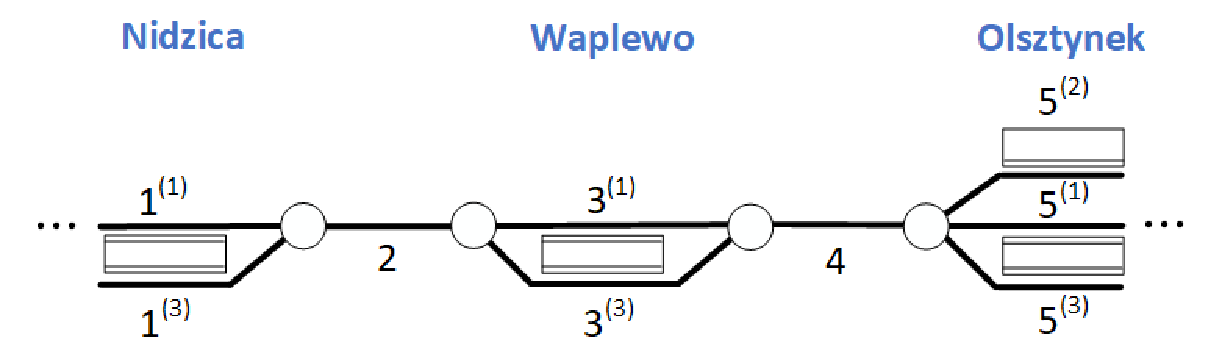
\includegraphics[width=\textwidth]{figures/line_small.pdf}
    \caption{ Nidzica -- Olsztynek segment of line No. 216.}
  \end{subfigure}
  \begin{subfigure}[b]{\textwidth}
    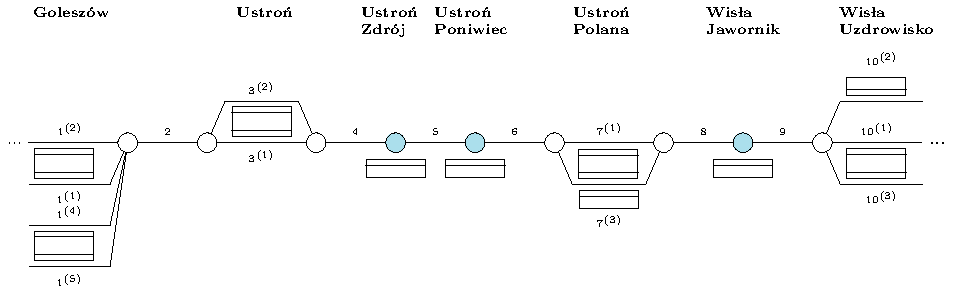
\includegraphics[width=\textwidth]{figures/line.pdf}
    \caption{Goleszów -- Wisła Uzdrowisko segment of railway line No. 191}
  \end{subfigure}
  \caption{
    Network segments studied in our work. The rectangles represent the passenger platforms,
    and the circles represent boundaries between line block and a station (white) or between
    two line blocks (blue).
  }
  \label{fig:railway-network}
\end{figure}

Both segments are depicted in Fig. \ref{fig:railway-network}
For the railway line No. 216, we considered its official train schedule (as of April 2020). The
line No. 191 was undergoing a renovation as of the time of writing, and hence it had no
available timetable. Based on the planned parameters of the line, as described in the official
documents \cite{}, we constructed a cyclic timetable. Both timetables are depicted in Fig.
\ref{fig:timetables}.

\begin{figure}
  \begin{subfigure}[t]{\textwidth}
	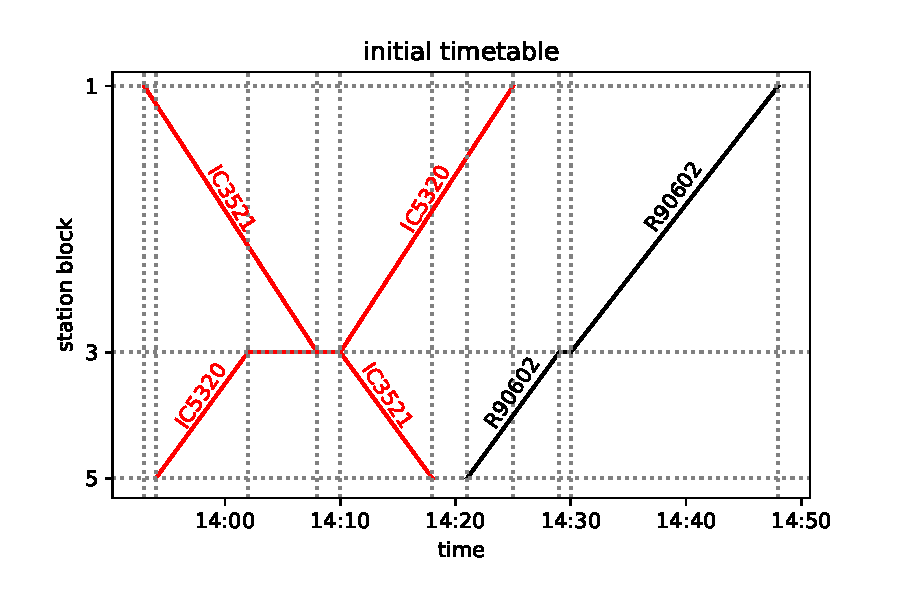
\includegraphics[width=\textwidth]{figures/train_diagram_small}
	\subcaption{Train diagram for the timetable of the line in Fig.~\ref{fig::small_line}}\label{fig::small_diagram}
  \end{subfigure}
  \begin{subfigure}[t]{\textwidth}
    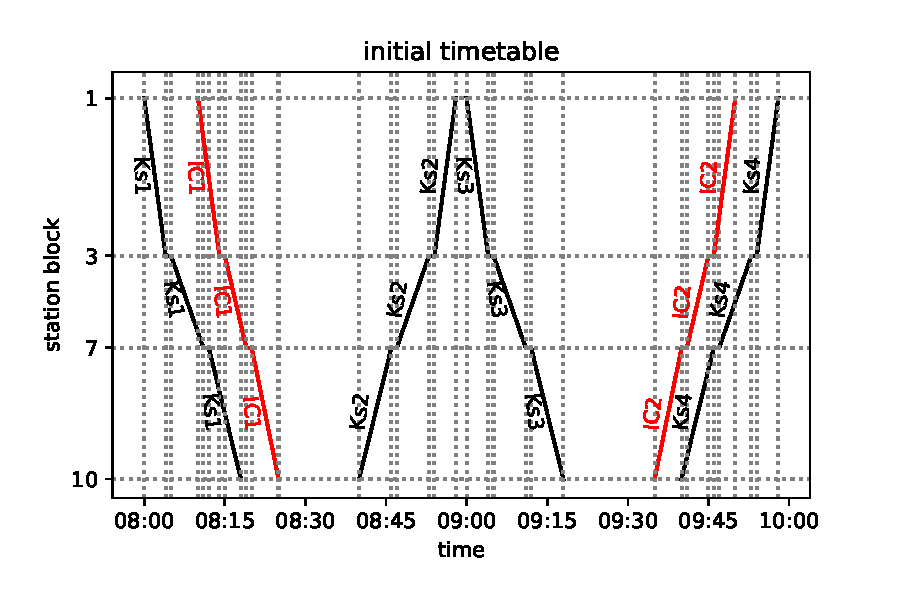
\includegraphics[width=\textwidth]{figures/train_diagram}
    \subcaption{Train diagram for the timetable of the line in
      Fig.~\ref{fig::line}}\label{fig::diagram}
  \end{subfigure}
  \caption{Train diagrams for the studies network segments.}
  \label{fig:timetables}
\end{figure}


%%% Local Variables:
%%% mode: latex
%%% TeX-master: "../main"
%%% End:
